\documentclass[12pt,]{article}
\usepackage{lmodern}
\usepackage{amssymb,amsmath}
\usepackage{ifxetex,ifluatex}
\usepackage{fixltx2e} % provides \textsubscript
\ifnum 0\ifxetex 1\fi\ifluatex 1\fi=0 % if pdftex
  \usepackage[T1]{fontenc}
  \usepackage[utf8]{inputenc}
\else % if luatex or xelatex
  \ifxetex
    \usepackage{mathspec}
  \else
    \usepackage{fontspec}
  \fi
  \defaultfontfeatures{Ligatures=TeX,Scale=MatchLowercase}
    \setmainfont[]{Times New Roman}
\fi
% use upquote if available, for straight quotes in verbatim environments
\IfFileExists{upquote.sty}{\usepackage{upquote}}{}
% use microtype if available
\IfFileExists{microtype.sty}{%
\usepackage{microtype}
\UseMicrotypeSet[protrusion]{basicmath} % disable protrusion for tt fonts
}{}
\usepackage[margin=2.54cm]{geometry}
\usepackage{hyperref}
\hypersetup{unicode=true,
            pdftitle={Examining the Relationship between Flow and Nutrient Levels at Upstream and Downstream Locations along Ellerbe Creek, North Carolina},
            pdfauthor={Rachel Landman},
            pdfborder={0 0 0},
            breaklinks=true}
\urlstyle{same}  % don't use monospace font for urls
\usepackage{longtable,booktabs}
\usepackage{graphicx,grffile}
\makeatletter
\def\maxwidth{\ifdim\Gin@nat@width>\linewidth\linewidth\else\Gin@nat@width\fi}
\def\maxheight{\ifdim\Gin@nat@height>\textheight\textheight\else\Gin@nat@height\fi}
\makeatother
% Scale images if necessary, so that they will not overflow the page
% margins by default, and it is still possible to overwrite the defaults
% using explicit options in \includegraphics[width, height, ...]{}
\setkeys{Gin}{width=\maxwidth,height=\maxheight,keepaspectratio}
\IfFileExists{parskip.sty}{%
\usepackage{parskip}
}{% else
\setlength{\parindent}{0pt}
\setlength{\parskip}{6pt plus 2pt minus 1pt}
}
\setlength{\emergencystretch}{3em}  % prevent overfull lines
\providecommand{\tightlist}{%
  \setlength{\itemsep}{0pt}\setlength{\parskip}{0pt}}
\setcounter{secnumdepth}{5}
% Redefines (sub)paragraphs to behave more like sections
\ifx\paragraph\undefined\else
\let\oldparagraph\paragraph
\renewcommand{\paragraph}[1]{\oldparagraph{#1}\mbox{}}
\fi
\ifx\subparagraph\undefined\else
\let\oldsubparagraph\subparagraph
\renewcommand{\subparagraph}[1]{\oldsubparagraph{#1}\mbox{}}
\fi

%%% Use protect on footnotes to avoid problems with footnotes in titles
\let\rmarkdownfootnote\footnote%
\def\footnote{\protect\rmarkdownfootnote}

%%% Change title format to be more compact
\usepackage{titling}

% Create subtitle command for use in maketitle
\providecommand{\subtitle}[1]{
  \posttitle{
    \begin{center}\large#1\end{center}
    }
}

\setlength{\droptitle}{-2em}

  \title{Examining the Relationship between Flow and Nutrient Levels at Upstream
and Downstream Locations along Ellerbe Creek, North Carolina}
    \pretitle{\vspace{\droptitle}\centering\huge}
  \posttitle{\par}
  \subtitle{\url{https://github.com/rml41/EDA_2020_Project.git}}
  \author{Rachel Landman}
    \preauthor{\centering\large\emph}
  \postauthor{\par}
    \date{}
    \predate{}\postdate{}
  

\begin{document}
\maketitle

\newpage
\tableofcontents 
\newpage
\listoftables 
\newpage
\listoffigures 
\newpage

\hypertarget{rationale-and-research-questions}{%
\section{Rationale and Research
Questions}\label{rationale-and-research-questions}}

Ellerbe Creek runs into the Falls Lake Resovoir, through the city of
Durham, North Carolina. Falls Lake serves as the source of drinking
water for the City of Raleigh and does not meet North Carolina standards
for \emph{chlorophyll a}, which is found in algae (SOURCE:
\url{https://durhamnc.gov/716/Falls-Lake}). Algal blooms generally come
from excess nutrients such as phosphorus and nitrogen. Ellerbe Creek is
one of the sources of excess nutrients and contaminents in Falls Lake.
The Ellerbe Creek Watershed has the highest population density of
Durham's watersheds, with an estimated 22\% impervious surface (SOURCE:
\url{https://files.nc.gov/ncdeq/Water\%20Quality/Planning/BPU/BPU/Neuse/Neuse\%20Plans/2009\%20Plan/Chapter\%201.pdf}).
It is impacted by both point and nonpoint sources and was found to
deliver the highest nutrient loads to Falls Lake (SOURCE:
\url{https://files.nc.gov/ncdeq/Water\%20Quality/Planning/BPU/BPU/Neuse/Neuse\%20Plans/2009\%20Plan/Chapter\%201.pdf}).
Ellerbe Creek and Falls Lake are both on the state's impaired water
bodies list (303(d) list) (SOURCE
\url{https://durhamnc.gov/711/Ellerbe-Creek-Watershed},
\url{https://www.usgs.gov/centers/sa-water/science/groundwatersurface-water-interaction-near-ellerbe-creek-durham-nc?qt-science_center_objects=0\#qt-science_center_objects}).
Ellerbe Creek was first listed on the 303(d) list in 1998 (SOURCE:
\url{https://files.nc.gov/ncdeq/Water\%20Quality/Planning/BPU/BPU/Neuse/Neuse\%20Plans/2009\%20Plan/Chapter\%201.pdf})

This analysis and report will aim to answer the following questions: 1.
Are Nitrogen and Phosphorus levels in Ellerbe Creek above recommended
levels? 2. Is there a relationship between flow and Nitrogen or
Phosphorus levels? 3. How does location, upstream vs.~downstream, impact
nutrient levels?

\newpage

\hypertarget{dataset-information}{%
\section{Dataset Information}\label{dataset-information}}

Nutrient data for this project were downloaded from the the Water
Quality Portal, a coorperative service sponsered by the United States
Geological Survey (USGS), the Environmental Protection Agency (EPA), and
the National Water Quality Monitoring Council (NWQMC) on February 27,
2020. Discharge data were downloaded for two stream gages along Ellerbe
Creek, HUC code 030202010403, from USGS using the data dataRetrieval
package in R. The dataset analyzed contains 21 monitoring locations with
measurments for nitrogen and phosphorus levels from 1982 to 2018 and
daily discharge data from 2008 to 20202. Not all locations had data for
each nutrient. Nitrogen and Phosphorus concentrations are recorded as
mg/L of Nitrogen or Phosphorus in various compounds including, nitrate,
nitrite, ammonia, ammonium, organic nitrogen, phosphate, and organic
phosphorus. The USGS gage locations are Club Blvd (0208675010),
upstream, and Gorman (02086849), downstream.

\begin{longtable}[]{@{}llllll@{}}
\toprule
Variable & Units & Range & Mean & Median & Source\tabularnewline
\midrule
\endhead
Nitrogen & mg/L N & 0.37 - 33.00 & 7.18 & 2.82 & NC DENR and
USGS\tabularnewline
Phosphorus & mg/L P & 0.039 - 17.00 & 1.091 & 0.157 & NC DENR and
USGS\tabularnewline
Discarge Club & ft\^{}3/s & 0.20 - 781.00 & 9.39 & 1.28 &
USGS\tabularnewline
Discharge Gorman & ft\^{}3/s & 7.52 - 1750.00 & 48.84 & 20.50 &
USGS\tabularnewline
\bottomrule
\end{longtable}

\newpage

\hypertarget{exploratory-analysis}{%
\section{Exploratory Analysis}\label{exploratory-analysis}}

\hypertarget{initial-exploration}{%
\subsection{Initial Exploration}\label{initial-exploration}}

Explored raw data from the water quality portal to determine potential
variables for analysis and time period of data. Examined a summary of
all the characteristics in the dataset to determine the count for each
variable. Selected Nitrogen, mixed forms (NH3), (NH4), organic, (NO2)
and (NO3) and Phosphorus as the two variables to analyze. Explored
discharge data to determine date range of data.

Table 2. Sample of summary results from raw data

\begin{longtable}[]{@{}ll@{}}
\toprule
Variable & Count\tabularnewline
\midrule
\endhead
Dissolved Oxygen & 636\tabularnewline
Nitrate & 128\tabularnewline
Nitrogen, mixed forms (NH3), (NH4), organic, (NO2) and (NO3) &
209\tabularnewline
Phosphorus & 286\tabularnewline
RBP Stream Width & 14\tabularnewline
Temperature, water & 1146\tabularnewline
Total Dissolved Solids & 278\tabularnewline
\bottomrule
\end{longtable}

\hypertarget{location-of-monitoring-sites}{%
\subsection{Location of Monitoring
Sites}\label{location-of-monitoring-sites}}

\begin{figure}
\centering
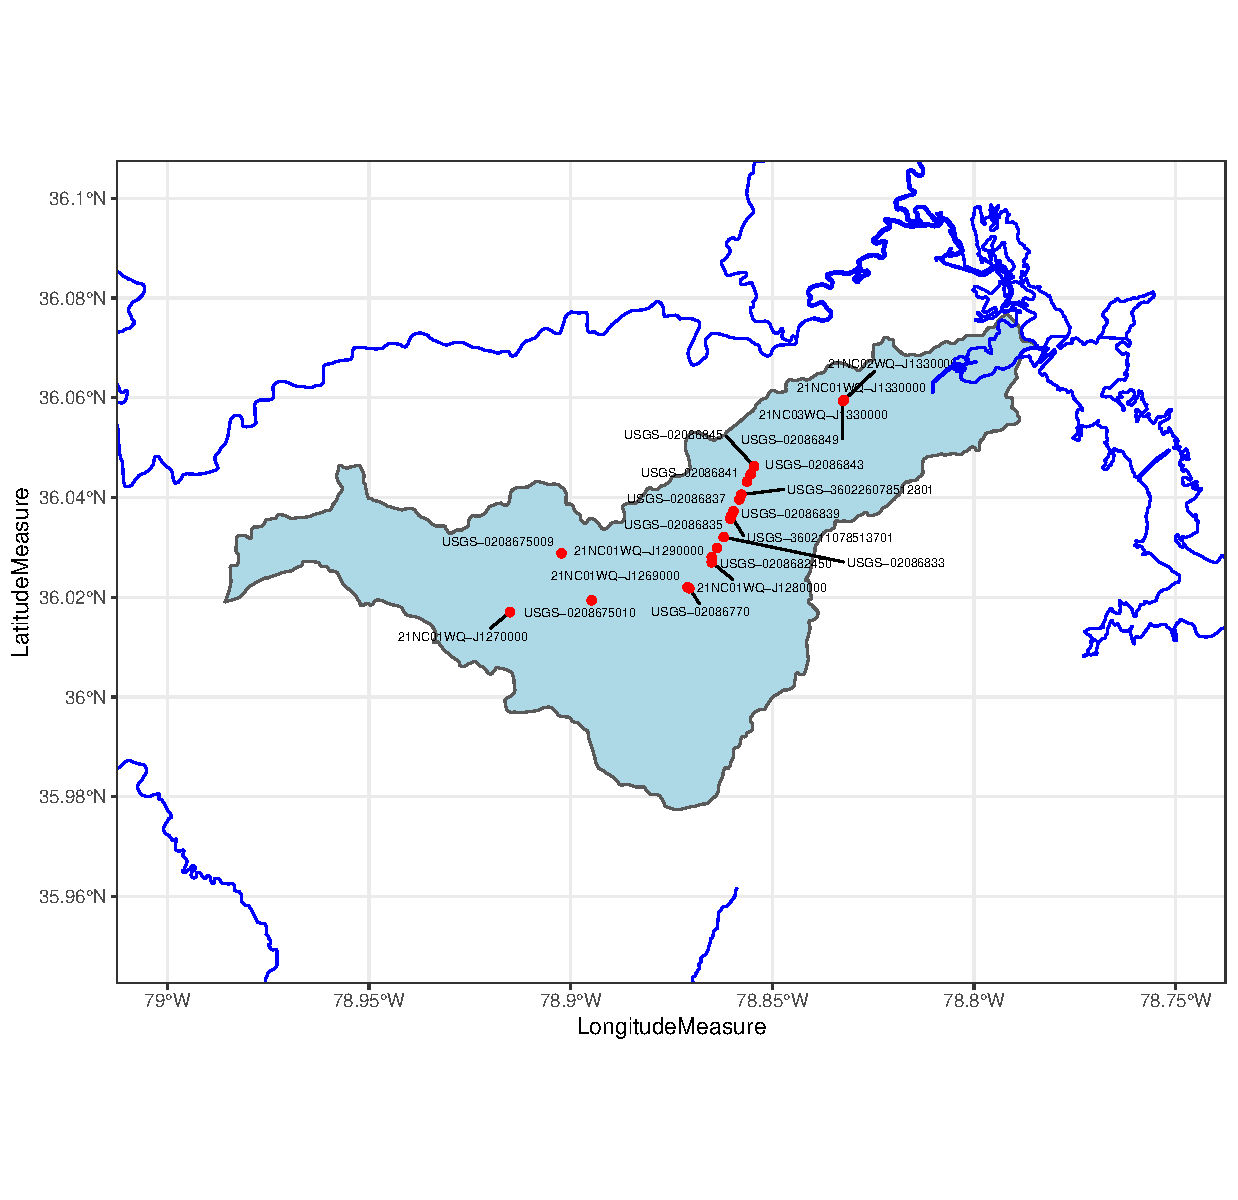
\includegraphics{Landman_ENV872_Project_files/figure-latex/Exploratory Analysis Figure 1-1.pdf}
\caption{Map of the Ellerbe Creek Watershed and Monitoring Locations
along Ellerbe Creek}
\end{figure}

\newpage

\hypertarget{discharge-data-wrangling}{%
\subsection{Discharge Data Wrangling}\label{discharge-data-wrangling}}

Flow data from the two USGS stream gages were combined in two data sets,
one as a long format with all discharge in one column and one in wide
format, with two seperate columns for discharge based on location.

\hypertarget{discharge-data-exploration}{%
\subsection{Discharge Data
Exploration}\label{discharge-data-exploration}}

A boxplot was made to visualize the range of discharge at each site

\begin{figure}
\centering
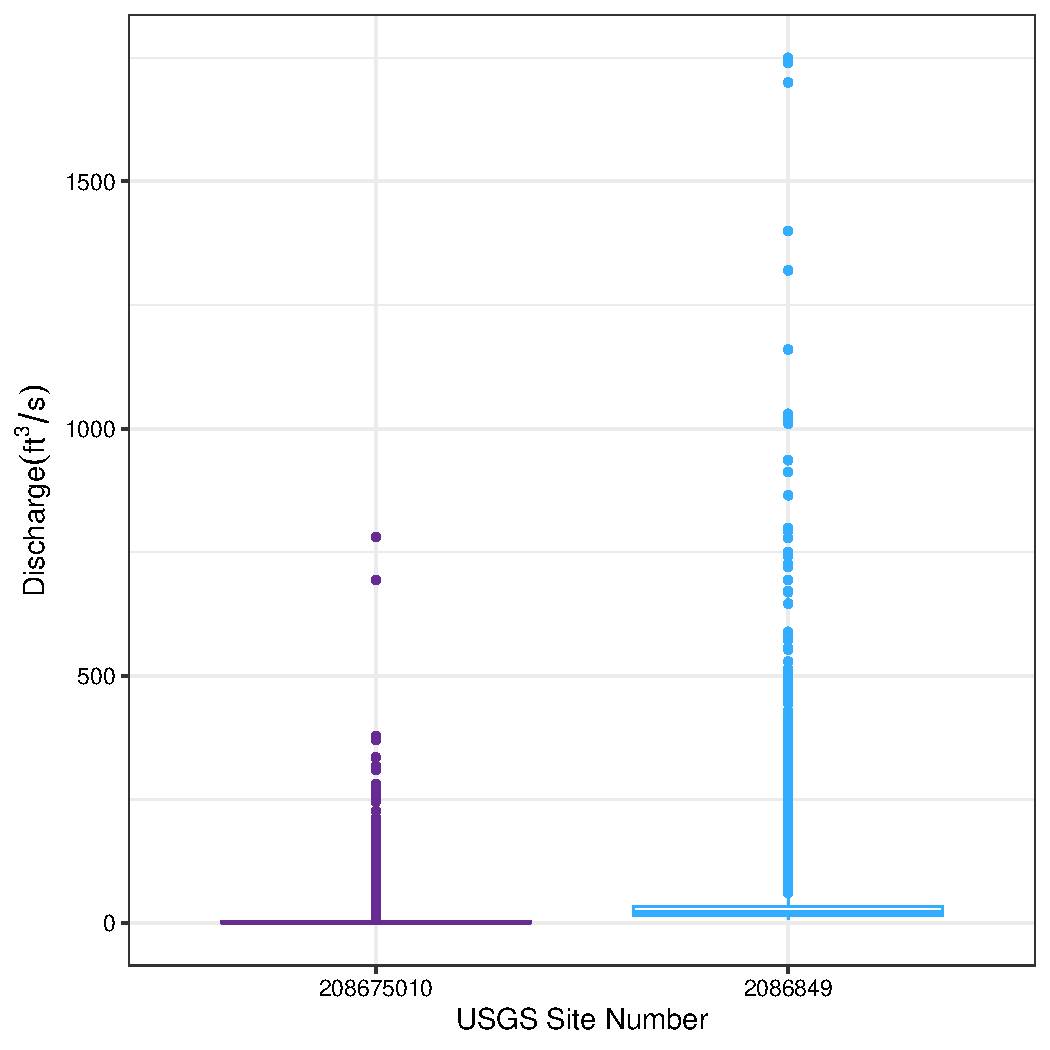
\includegraphics{Landman_ENV872_Project_files/figure-latex/Exploratory Analysis Figure 2-1.pdf}
\caption{Distribution of discharge at two sites, upstream (208675010)
and downstream (2086849) along Ellerbe Creek from January 1, 2008 to
April 17, 2020}
\end{figure}

\newpage

The discharge over time at each location does not show any obvious
seasonal or annual trends.

\begin{figure}
\centering
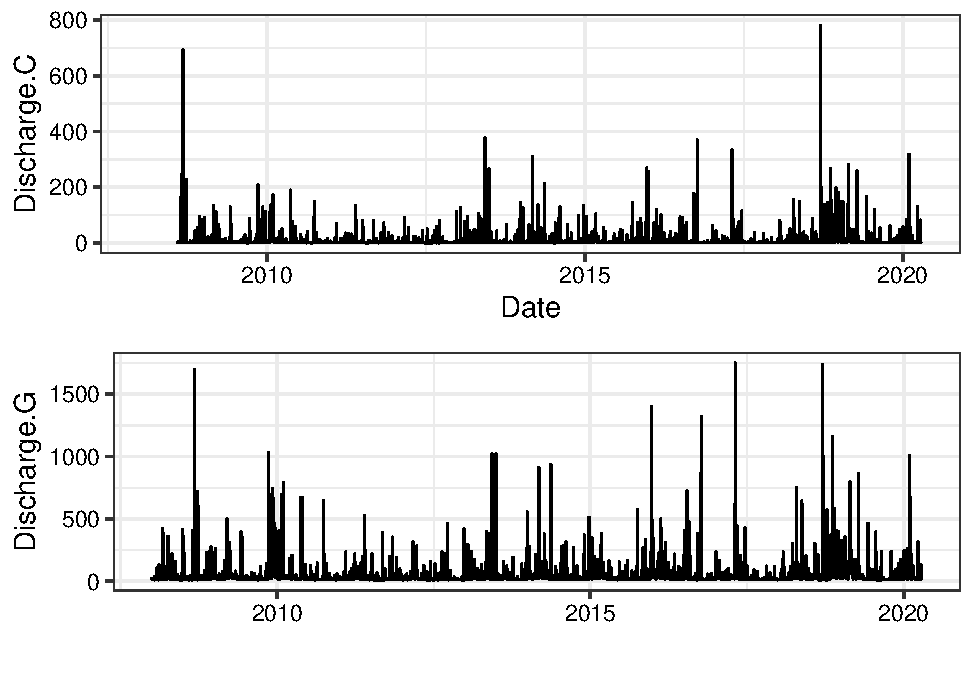
\includegraphics{Landman_ENV872_Project_files/figure-latex/Exploratory Analysis Figure 3-1.pdf}
\caption{Daily discharge at along Ellerbe Creek from January 1, 2008 to
April 17, 2020}
\end{figure}

\newpage

\hypertarget{nutrient-data-wrangling}{%
\subsection{Nutrient Data Wrangling}\label{nutrient-data-wrangling}}

The nutrient data set from the water quality portal was cleans to remove
all irrelevant information and retain just characterstics of interest,
Nitrogen and Phosphorus. Nitrogen and Phosphorus values for many samples
were recorded as both mg/L of N and P, and of NO3 and PO4 respectively.
Data were downloaded in long format and were converted to wide format in
order to convert Nitrogen and Phosphorus values to mg/L of N or P.
Relevant columns such as data, location, hydrologic event, variable
name, measured value, and units were selected and processed data were
saved as both long and wide format.

\hypertarget{nutrient-data-exploration}{%
\subsection{Nutrient Data Exploration}\label{nutrient-data-exploration}}

\begin{figure}
\centering
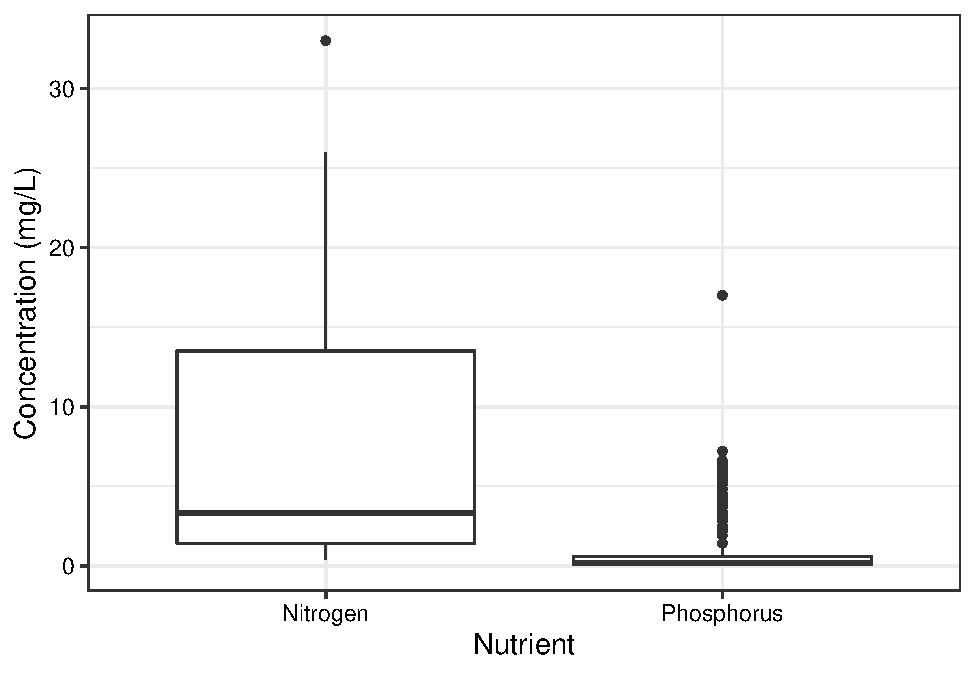
\includegraphics{Landman_ENV872_Project_files/figure-latex/Exploratory Analysis Figure 4-1.pdf}
\caption{Distribution of Nitrogen and Phosphorus Concentrations in
Ellerbe Creek from November 17, 1982 to December 17, 2018}
\end{figure}

\newpage

\begin{figure}
\centering
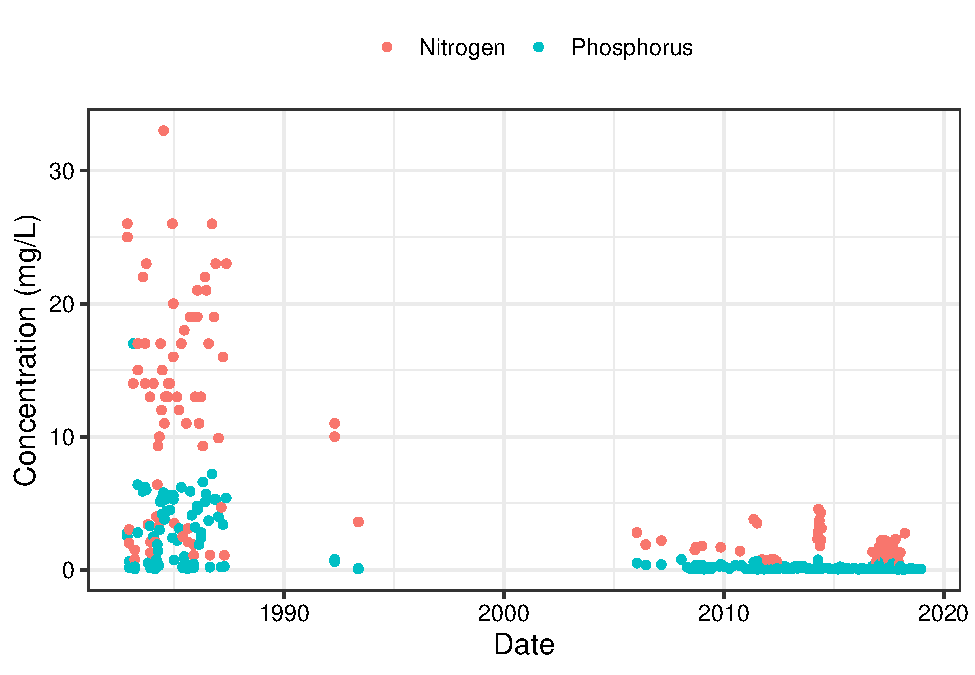
\includegraphics{Landman_ENV872_Project_files/figure-latex/Exploratory Analysis Figure 5-1.pdf}
\caption{Concentrations of Nitrogen and Phosphorus over Time in Ellerbe
Creek from November 17, 1982 to December 17, 2018}
\end{figure}

\newpage

\hypertarget{analysis}{%
\section{Analysis}\label{analysis}}

\hypertarget{question-1-are-nitrogen-and-phosphorus-levels-in-ellerbe-creek-above-recommended-levels}{%
\subsection{Question 1: Are Nitrogen and Phosphorus levels in Ellerbe
Creek above recommended
levels?}\label{question-1-are-nitrogen-and-phosphorus-levels-in-ellerbe-creek-above-recommended-levels}}

\begin{longtable}[]{@{}rrrrrrrr@{}}
\caption{Total Nitrogen and Phosphorus Conentrations}\tabularnewline
\toprule
mean.N & min.N & max.N & Standard.dev.N & mean.P & min.P & max.P &
Standard.dev.P\tabularnewline
\midrule
\endfirsthead
\toprule
mean.N & min.N & max.N & Standard.dev.N & mean.P & min.P & max.P &
Standard.dev.P\tabularnewline
\midrule
\endhead
7.183095 & 0.37 & 33 & 7.773407 & 1.091398 & 0.039 & 17 &
2.082384\tabularnewline
\bottomrule
\end{longtable}

\newpage

\begin{figure}
\centering
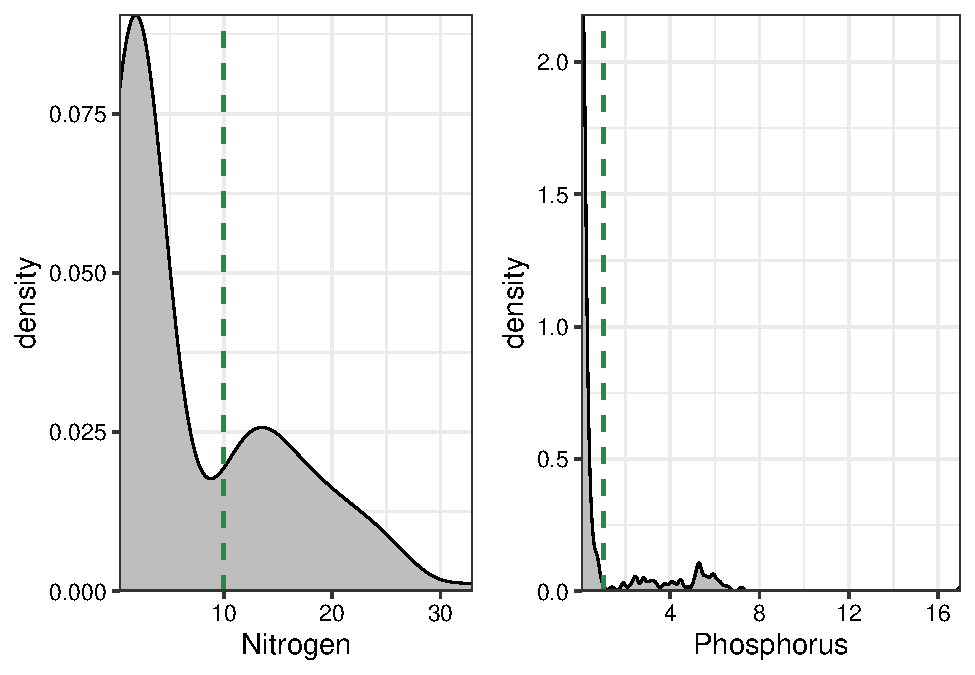
\includegraphics{Landman_ENV872_Project_files/figure-latex/Data Analysis Figure 6-1.pdf}
\caption{Density plots of Nitrogen and Phosphorus Concentrations}
\end{figure}

\newpage

\hypertarget{question-2-is-there-a-relationship-between-flow-and-nitrogen-or-phosphorus-levels}{%
\subsection{Question 2: Is there a relationship between flow and
Nitrogen or Phosphorus
levels?}\label{question-2-is-there-a-relationship-between-flow-and-nitrogen-or-phosphorus-levels}}

\begin{figure}
\centering
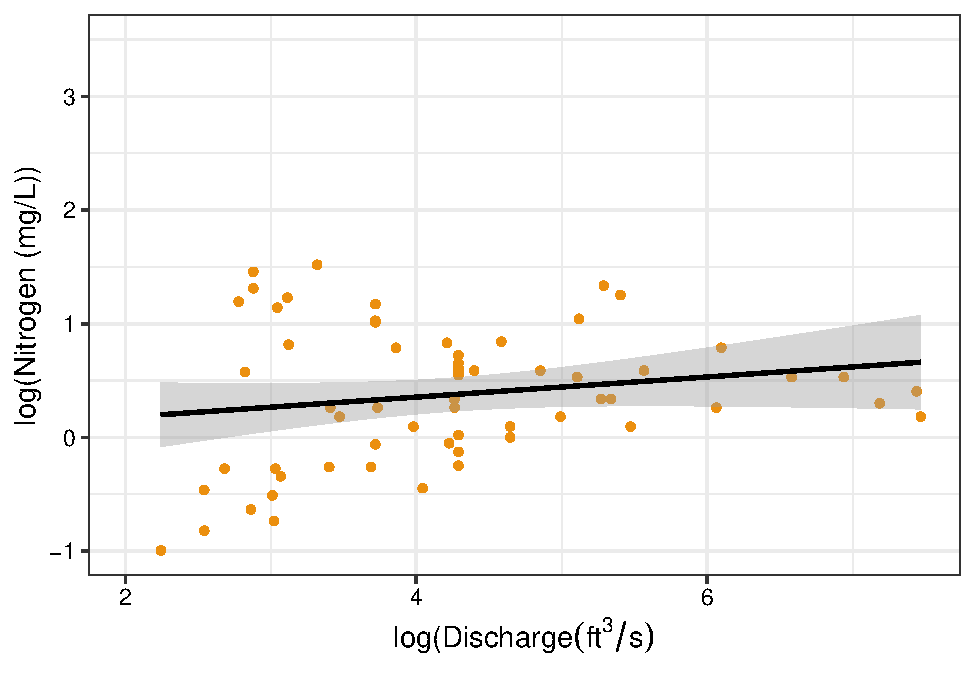
\includegraphics{Landman_ENV872_Project_files/figure-latex/Data Analysis Figure 7-1.pdf}
\caption{Linear regression of the log of Nitrogen Concentration vs.~the
log of Discharge}
\end{figure}

\begin{figure}
\centering
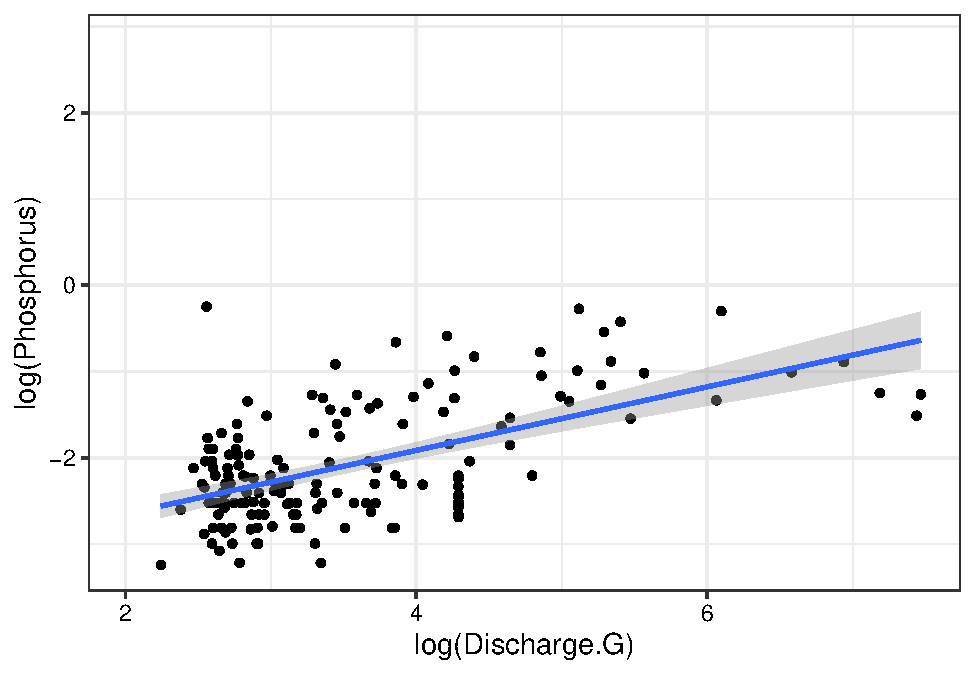
\includegraphics{Landman_ENV872_Project_files/figure-latex/Data Analysis Figure 8-1.pdf}
\caption{Linear regression of the log of Phosphorus Concentration
vs.~the log of Discharge}
\end{figure}

\newpage

\hypertarget{question-3-how-does-location-upstream-vs.downstream-impact-nutrient-levels}{%
\subsection{Question 3: How does location, upstream vs.~downstream,
impact nutrient
levels?}\label{question-3-how-does-location-upstream-vs.downstream-impact-nutrient-levels}}

\begin{longtable}[]{@{}rrrrrrrr@{}}
\caption{Nitrogen and Phosphorus conentrations by
Location}\tabularnewline
\toprule
mean.N & min.N & max.N & Standard.dev.N & mean.P & min.P & max.P &
Standard.dev.P\tabularnewline
\midrule
\endfirsthead
\toprule
mean.N & min.N & max.N & Standard.dev.N & mean.P & min.P & max.P &
Standard.dev.P\tabularnewline
\midrule
\endhead
7.740577 & 0.37 & 33 & 7.952157 & 1.134506 & 0.039 & 17 &
2.116099\tabularnewline
\bottomrule
\end{longtable}

\begin{figure}
\centering
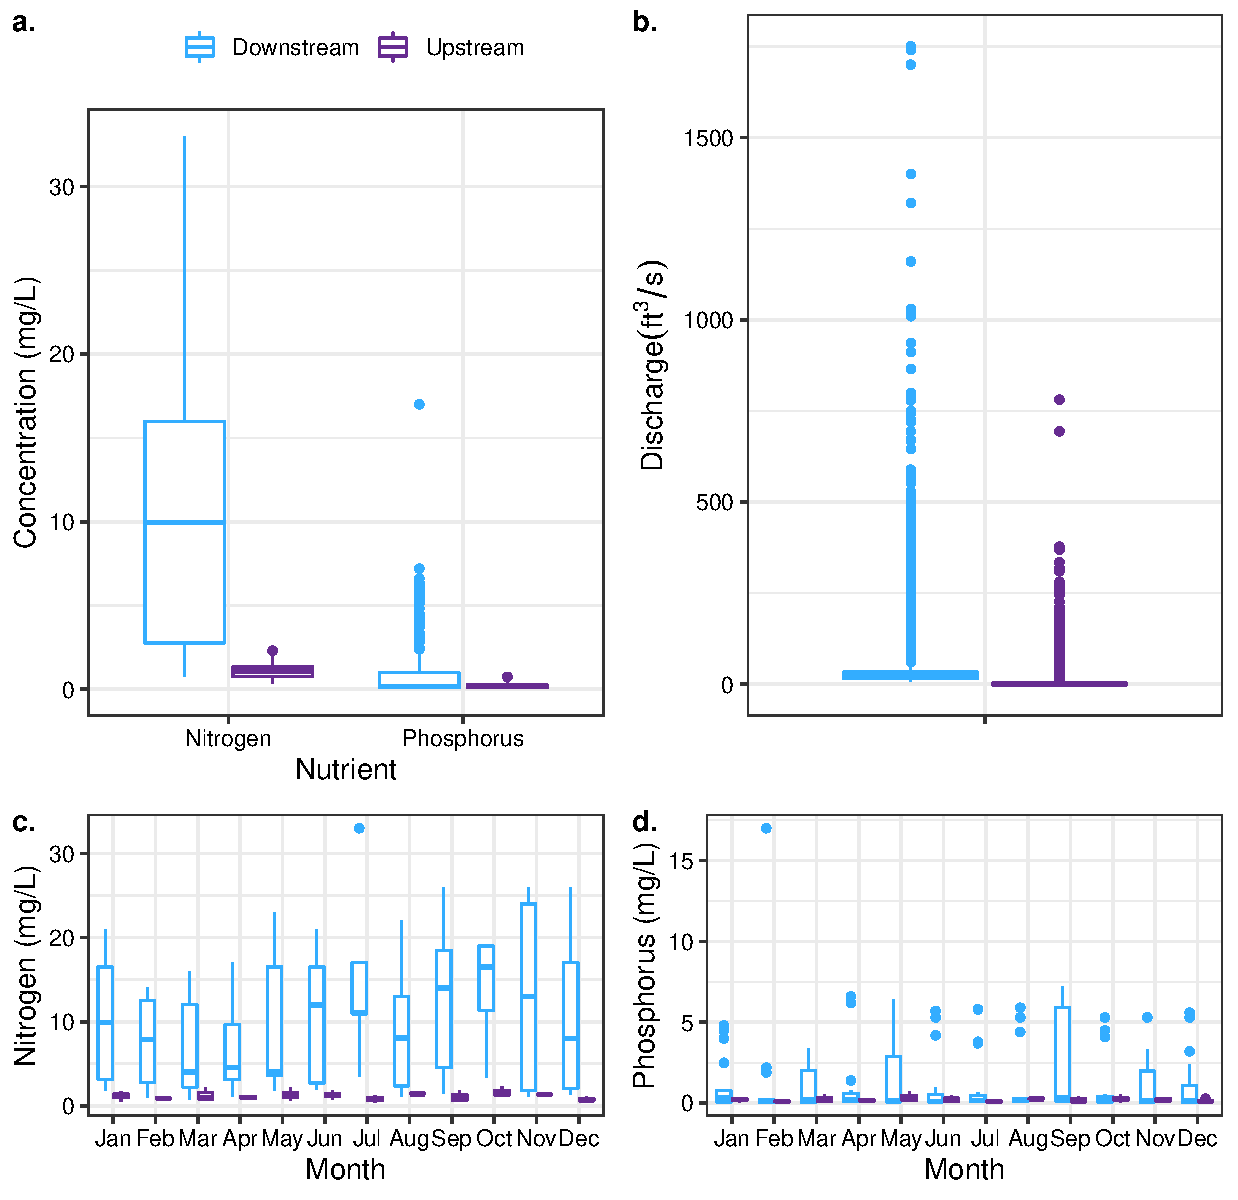
\includegraphics{Landman_ENV872_Project_files/figure-latex/Data Analysis Figure 9-1.pdf}
\caption{Distributions of nutrient concentrations and flow at upstream
and downstream monitoring sites along Ellerbe Creek in North Carolina.
a) Nitrogen and phosphorus concentrations at upstream and downstream
monitoring sites. b) Flow at upstream and downstream monitoring sites.
c) and d) Monthly distributions of nitrogen and phosphorus
concentrations at upstream and downstream monitoring sites.}
\end{figure}

\newpage

\hypertarget{summary-and-conclusions}{%
\section{Summary and Conclusions}\label{summary-and-conclusions}}

\newpage

\hypertarget{references}{%
\section{References}\label{references}}

\textless{}add references here if relevant, otherwise delete this
section\textgreater{}


\end{document}
